%%This is a very basic article template.
%%There is just one section and two subsections.
\documentclass[t]{beamer}

    \usepackage{multicol}

    \newcommand{\nologo}{\setbeamertemplate{logo}{}} %no logo on page 1
    
    \setbeamertemplate{caption}{\raggedright\insertcaption\par} %include figure #s

    \title{Text Time: The Terrific Timekiller \\ (CMPS183 Final Project)}
    \author{Cassia Artanegara, Jacob Runyan, Shane Kennerly}
    \institute{Jack Baskin School of Engineering \\ University of California, Santa Cruz}
    \date{June 11, 2018}
    \titlegraphic{
\includegraphics[scale=.06]{data/ucsc-logo.png}}
    \logo{
\includegraphics[width=1.5cm]{data/baskin-logo.png}}
    
    \begin{document}
    
    %special title page with no logo.
    {
    \nologo
    \begin{frame}
    \maketitle
    \end{frame}
    }

    \begin{frame}
        \frametitle{Why'd We Make It?}
        \begin{itemize}
          \item Simple game website for private and public games
          \item Base framework to add and recall games from
          \item But simply put...
        \end{itemize}
    \end{frame}

    \begin{frame}
        \frametitle{Why'd We Make It?}
        \begin{itemize}
          \item Simple game website for private and public games
          \item Base framework to add and recall games from
          \item But simply put...
          \item Our target audience is all you SLACKERS out there in lecture
        \end{itemize}
        \begin{figure}
            \begin{center}
                \fbox{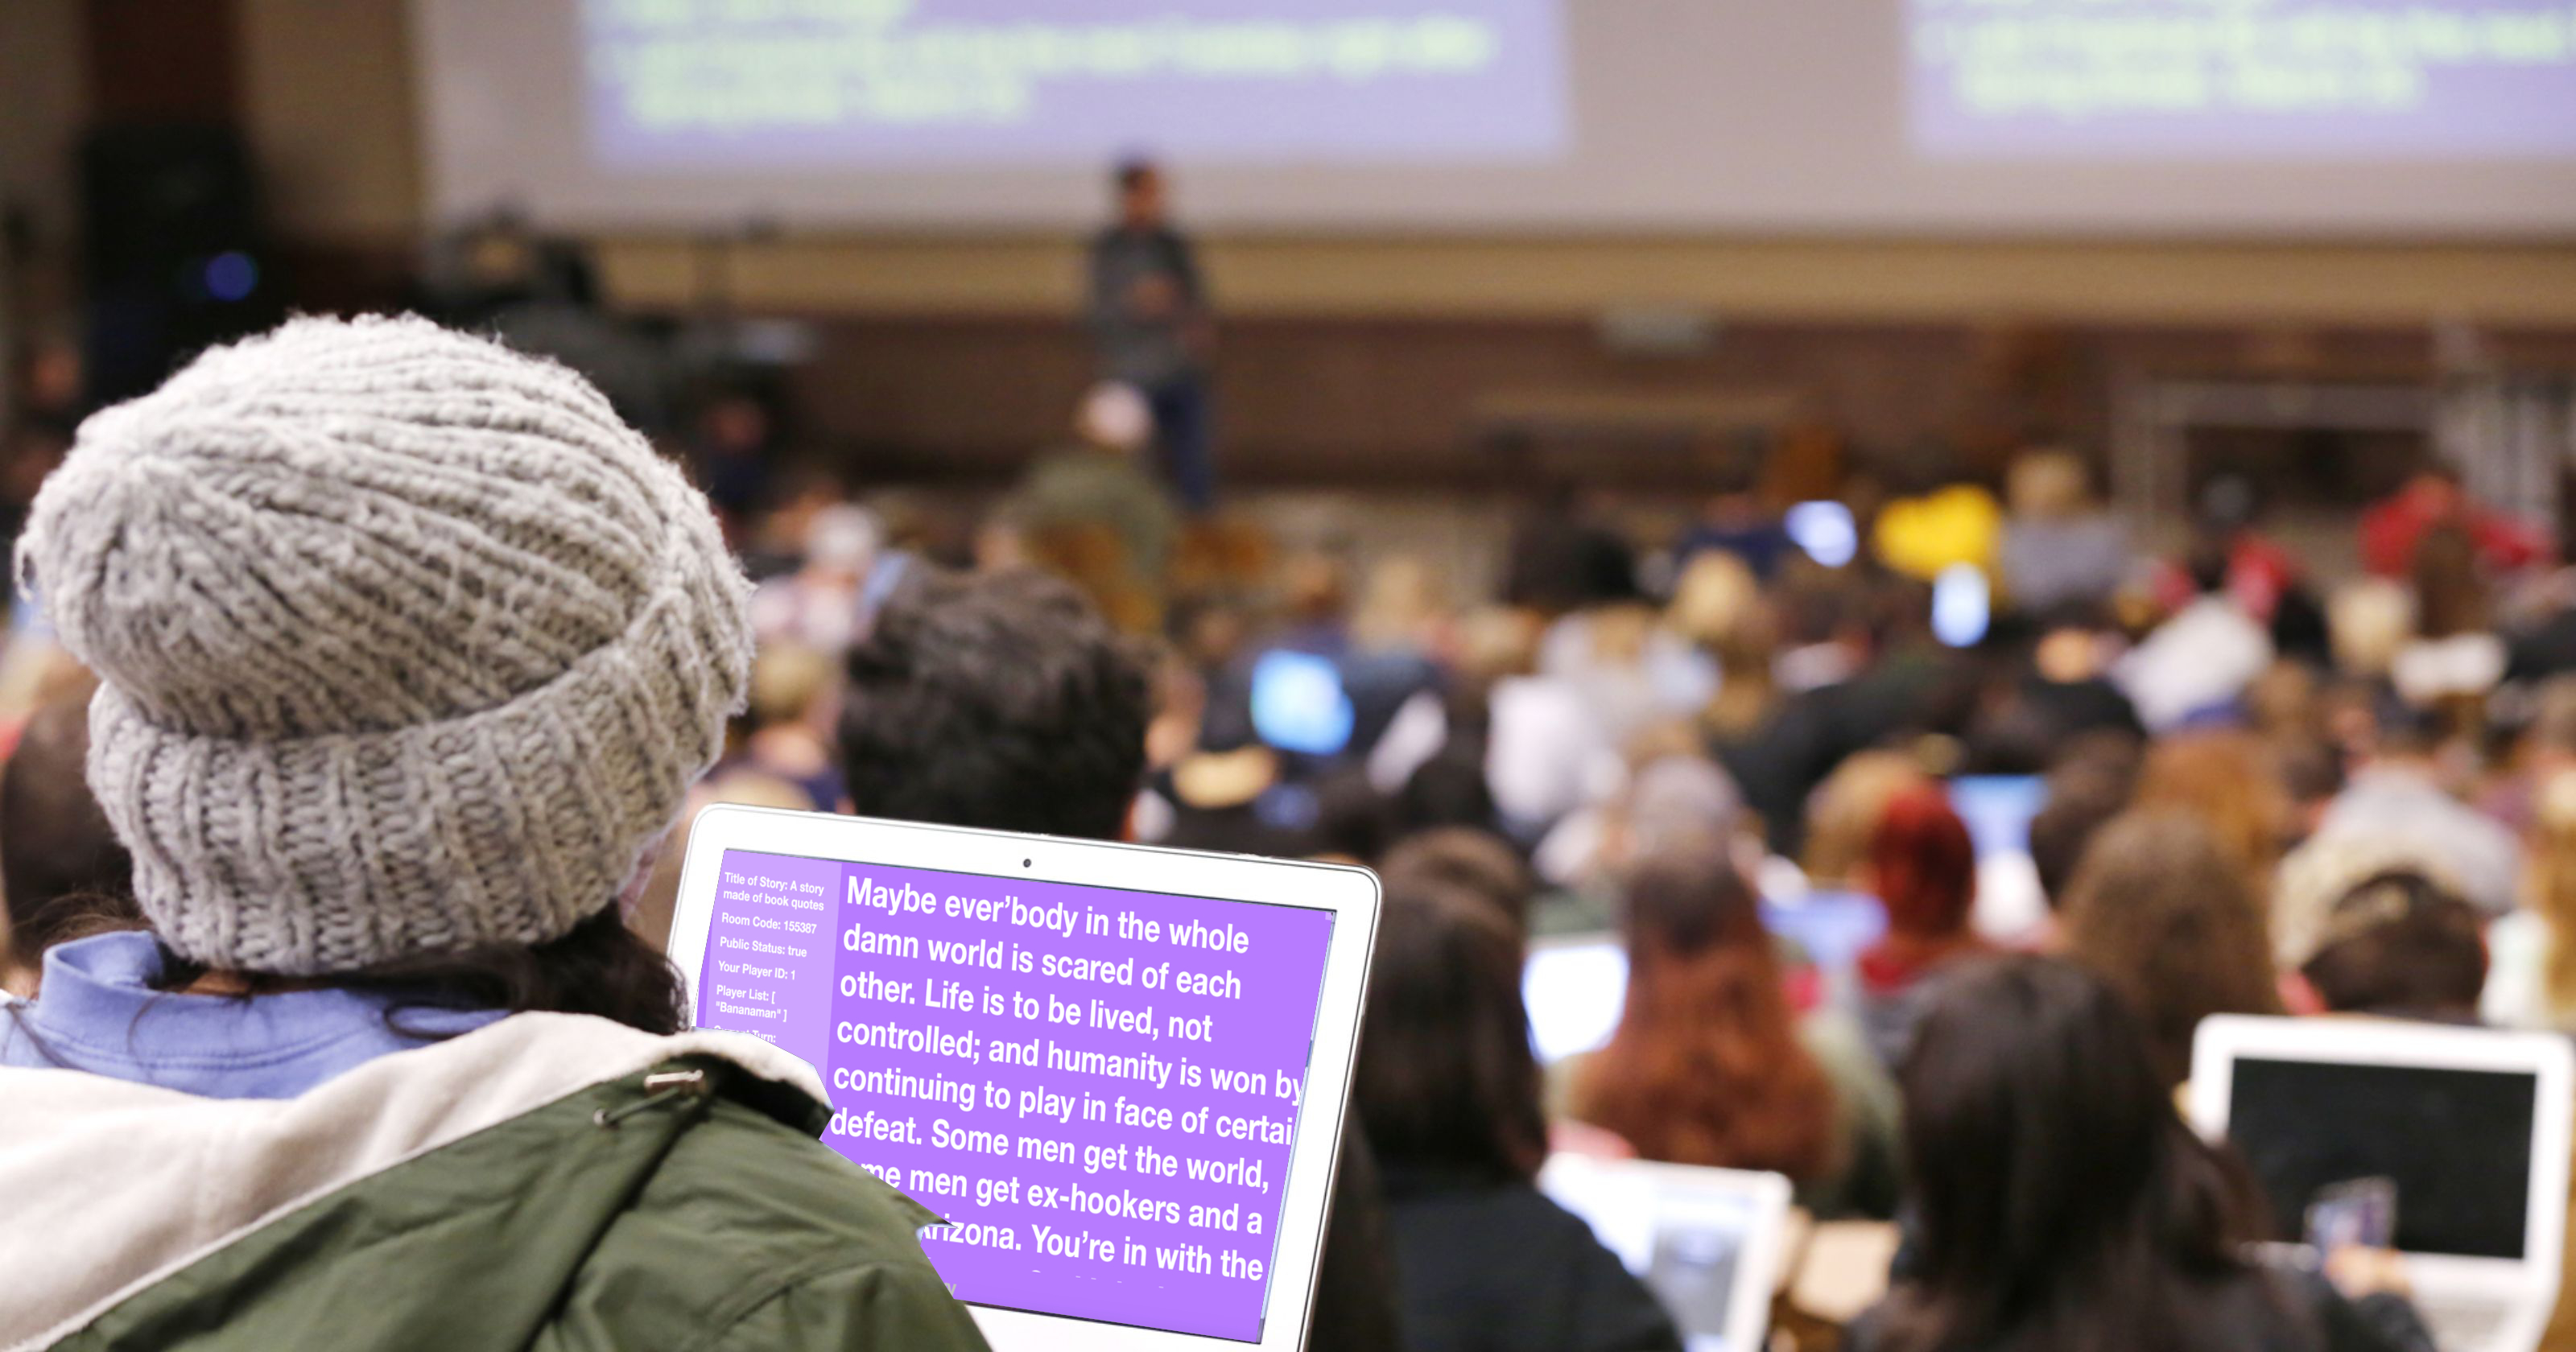
\includegraphics[width=200px]{data/talltalesinlecture.jpg}}
            \end{center}
            \caption{A student partakes in Tall Tales while in lecture}
        \end{figure}
    \end{frame}

    \begin{frame}
        \frametitle{Tall Tales, Our Communal Storybuilder}
        \begin{itemize}
          \item hoster creates a public or private game
          \begin{itemize}
            \item private games joinable by room code
            \item public games are viewable and joinable
          \end{itemize}
          \item players add sentences to a growing story 
          \item tell a story together or chat with friends
        \end{itemize}
        \begin{figure}
            \begin{center}
                \fbox{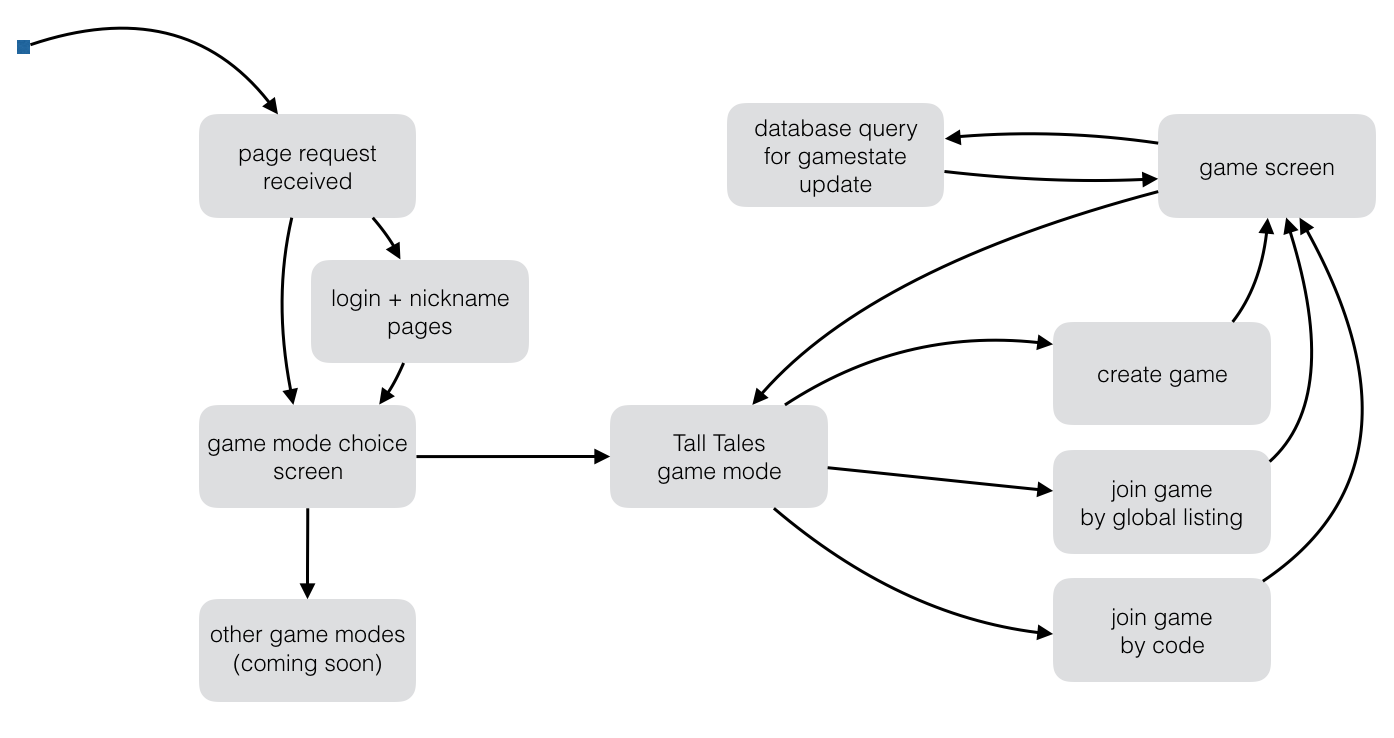
\includegraphics[width=200px]{data/htmlflow.png}}
            \end{center}
            \caption{Text Time's HTML flowchart}
        \end{figure}
    \end{frame}

    \begin{frame}
        \frametitle{Our Back-End and Front-End Wizardry}
        \begin{itemize}
          \item In the Back-End...
          \begin{itemize}
              \item database interaction achieved with AJAX requests to API
              \item database schema includes tables for gamestate, user customization options, and game-related text storage
          \end{itemize}
          \item And on the Front-End...
          \begin{itemize}
            \item vue.js maintains and updates gamestate, user, and page status information
            \item gamestates are updated with repeated AJAX requests to API
          \end{itemize}
        \end{itemize}
        \begin{figure}
            \begin{center}
                \fbox{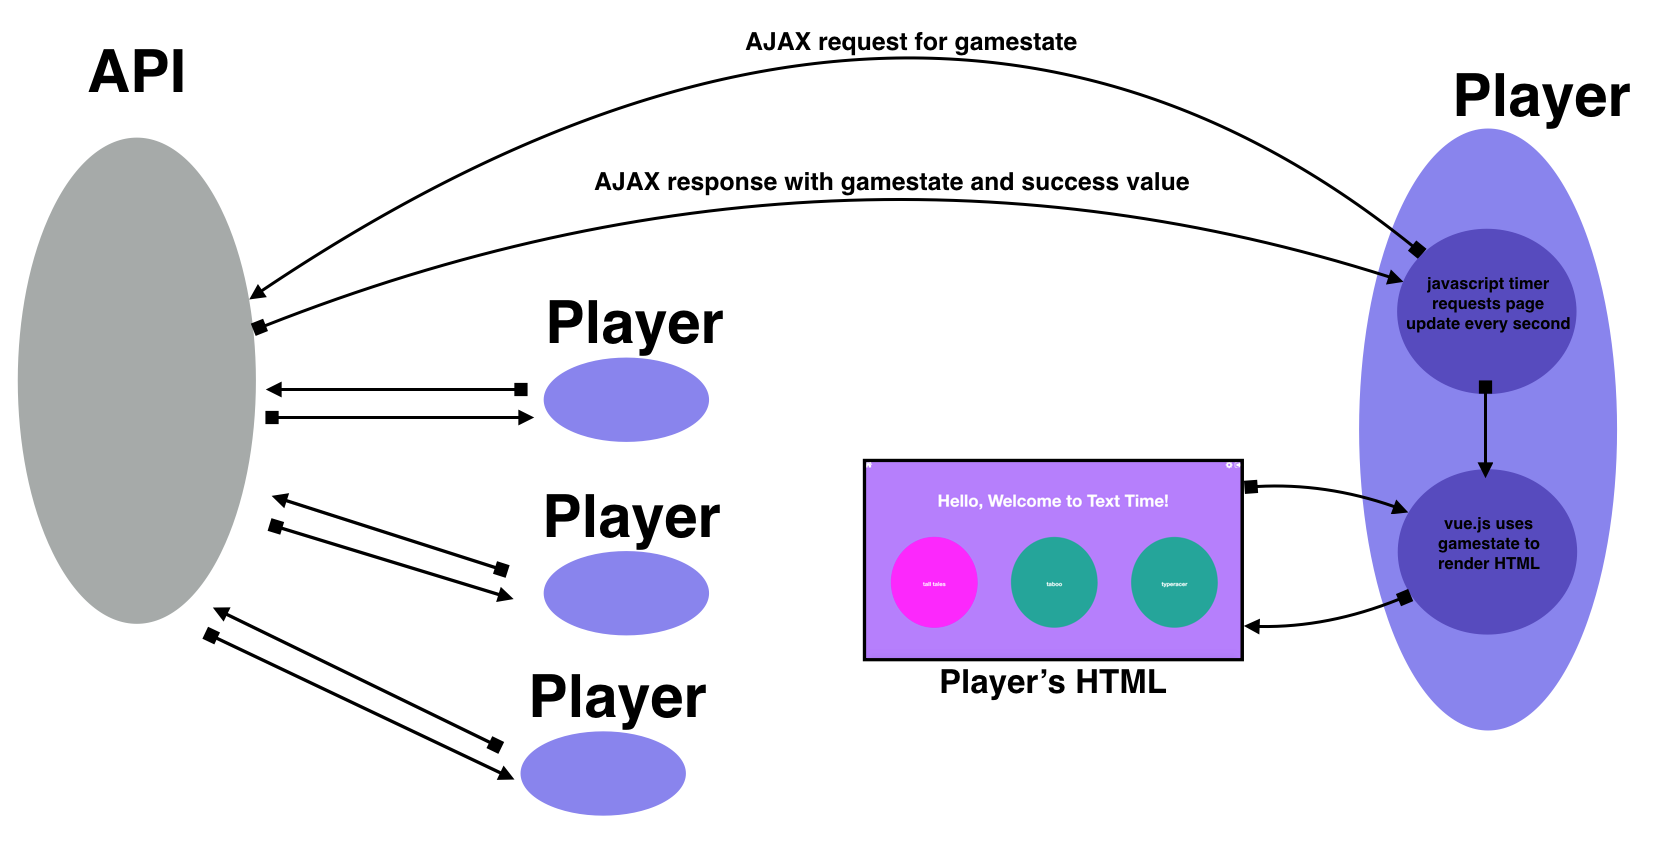
\includegraphics[width=200px]{data/apiflow.png}}
            \end{center}
            \caption{Text Time's API mockup}
        \end{figure}
    \end{frame}

    \begin{frame}
        \frametitle{Demo Time!}
        \begin{figure}
            \begin{center}
                \fbox{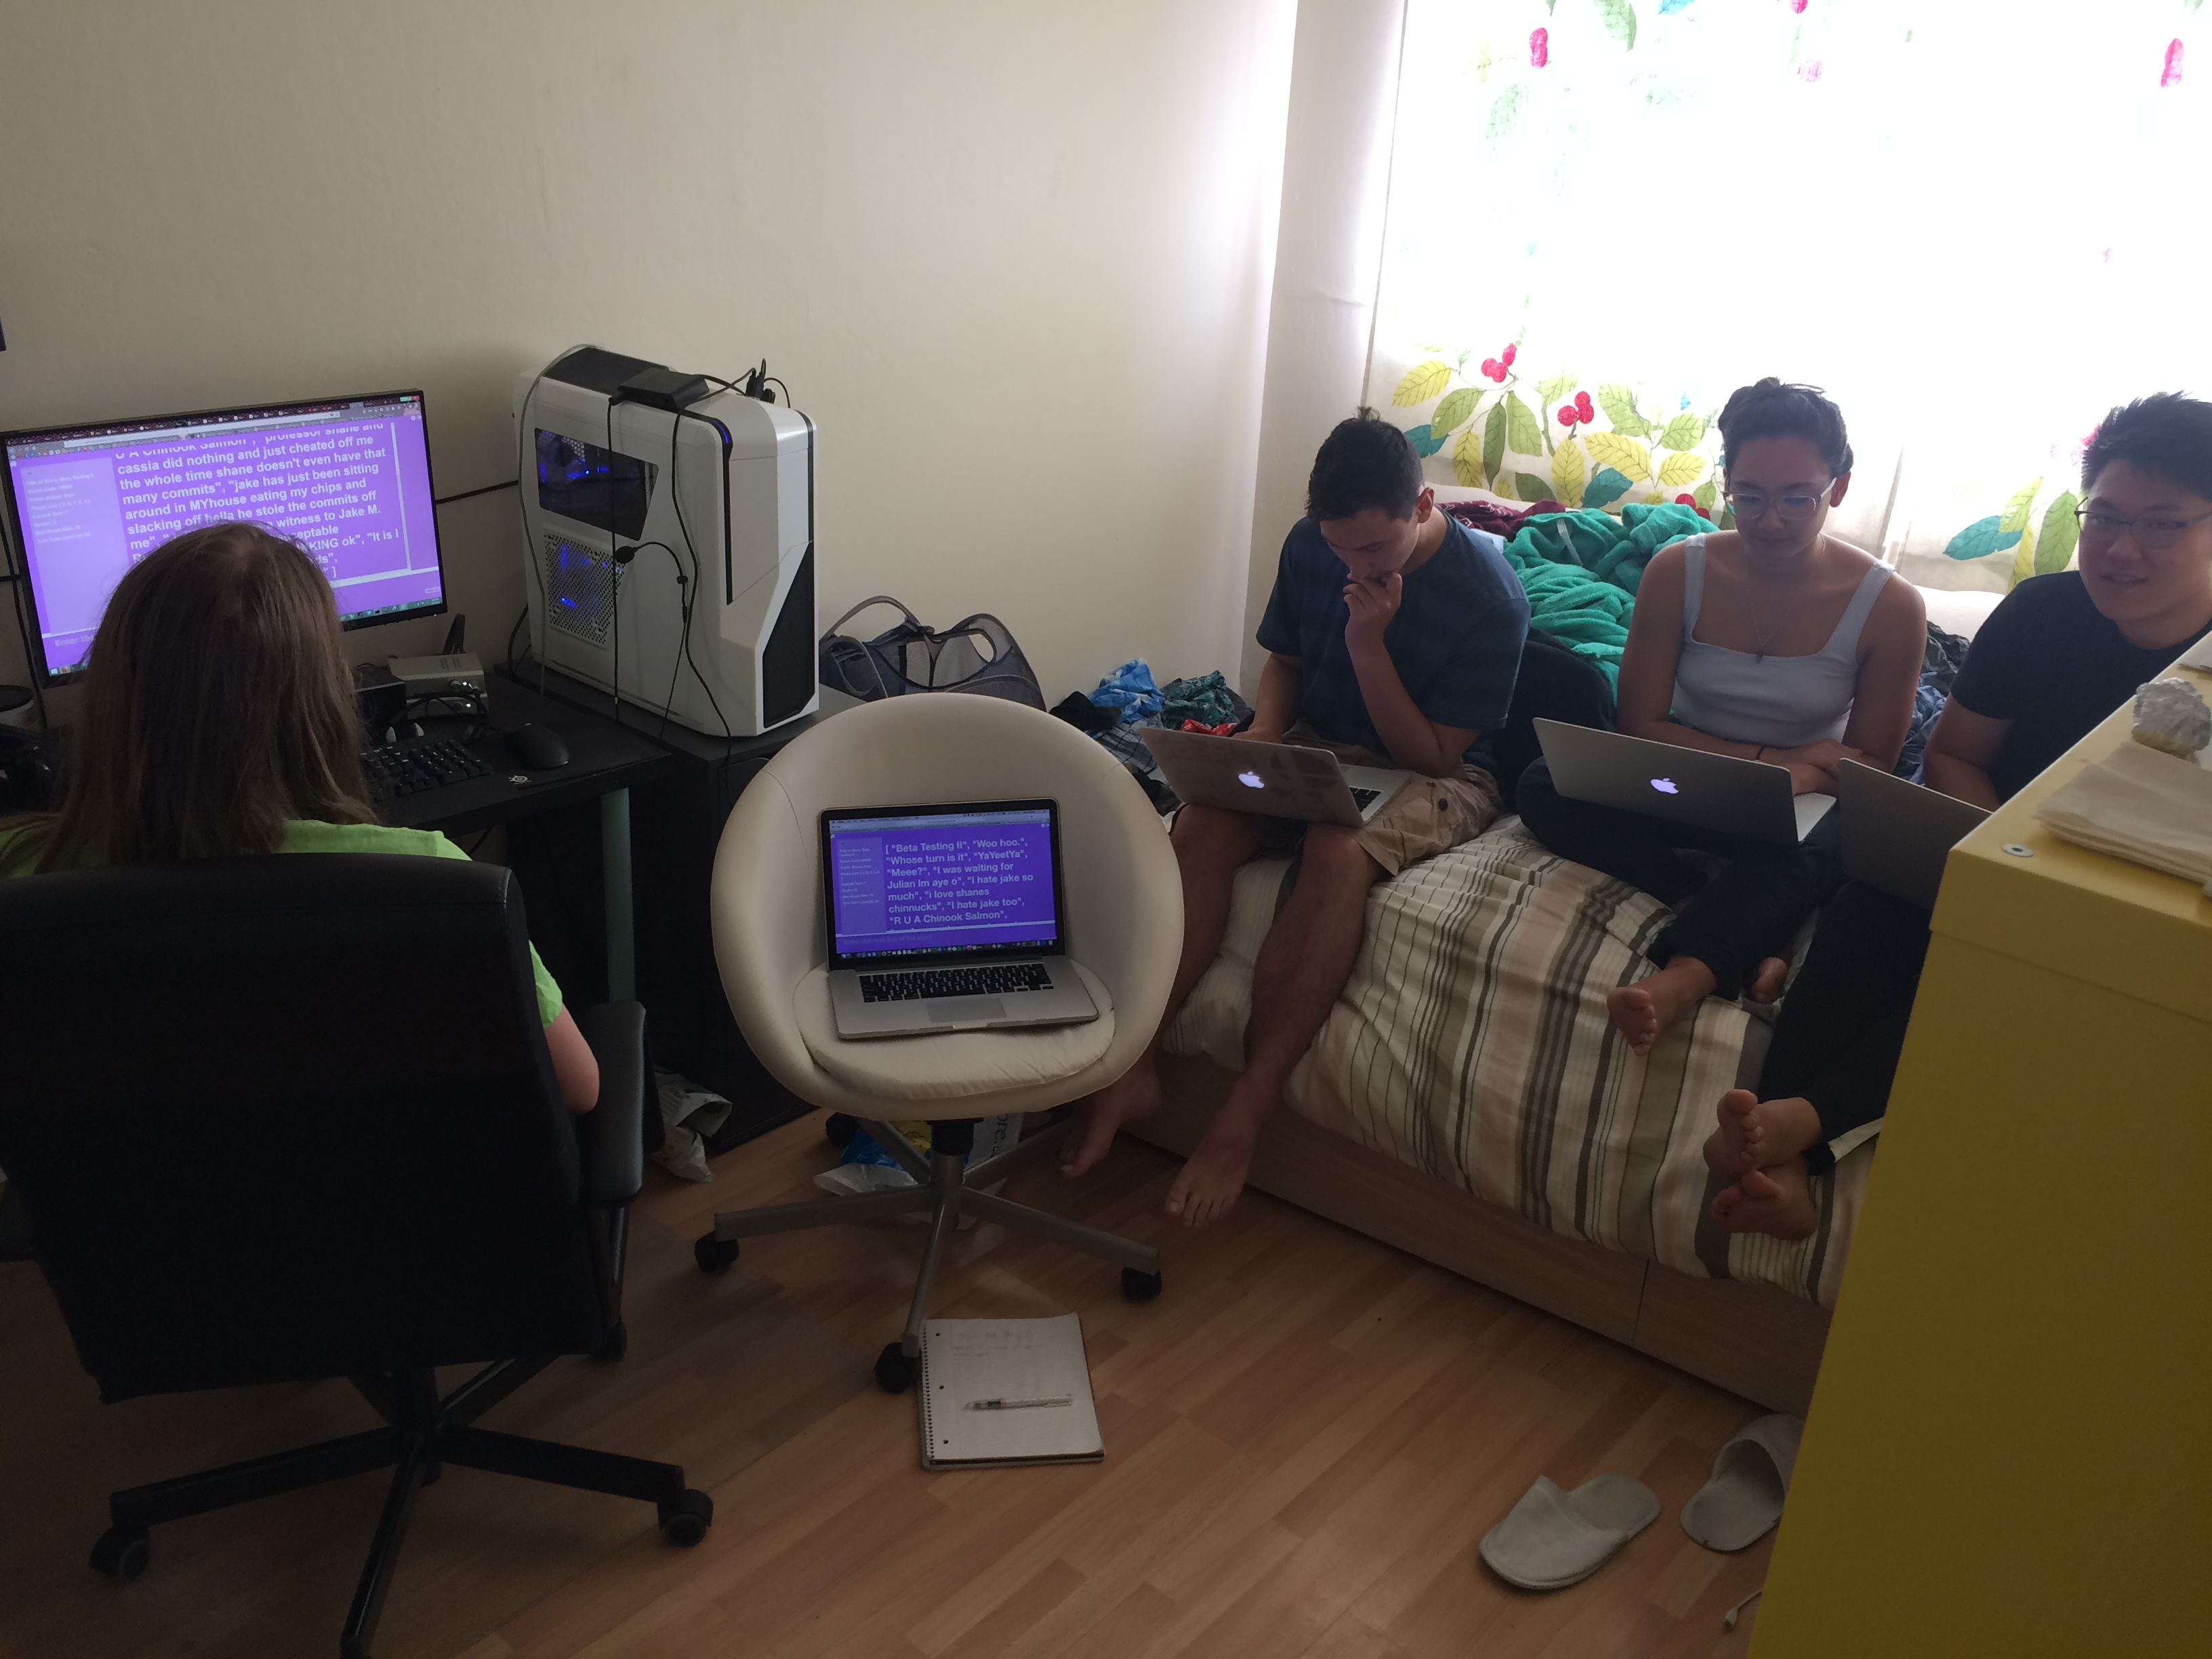
\includegraphics[width=200px]{data/betaii.jpg}}
            \end{center}
            \caption{A historical look at our first beta test}
        \end{figure}
    \end{frame}

    \begin{frame}
        \frametitle{The Road was Rocky....}
        \begin{itemize}
            \item Finalizing a first working game
            \begin{itemize}
                \item designing game flow regarding JS and API querying
                \item ensuring constant gamestates for local users, remote users, and API
                \item edge case testing for leaving game methods to minimize database leakage
            \end{itemize}
            \item Styling with user preferences
            \begin{itemize}
                \item resolved unclear UX areas using iterative beta testing
                \item finding reputable way to perform JS and HTML updates simultaneously
            \end{itemize}
            \item Generalizing our API for future games
            \begin{itemize}
                \item combination of \fbox{auth\_user} and our user customization table
                \item generalizing API for supplementary game modes
                \item resolving race conditions between HTML vue references and AJAX requests on page loading
            \end{itemize}
          \end{itemize}
    \end{frame}

    \begin{frame}
        \frametitle{The Future of Text Time}
        \begin{itemize}
            \item We plan to fully generalize our code base and implement other games
            \item Reduce network load of repeated querying when game window not focused
            \item Continual CSS updates for user convenience
            \item We plan to continue hosting via pythonanywhere
            \item Implementing some support system to submit error tickets
        \end{itemize}
    \end{frame}

    \begin{frame}
        \frametitle{References and Live Site}
        \begin{itemize}
          \item See our project live at: https://jmrunyan.pythonanywhere.com/texttime/
          \item Check out our code and cool README at: https://github.com/runyanjake/CJS-183-FinalProj
        \end{itemize}
        \begin{figure}
            \begin{center}
                \fbox{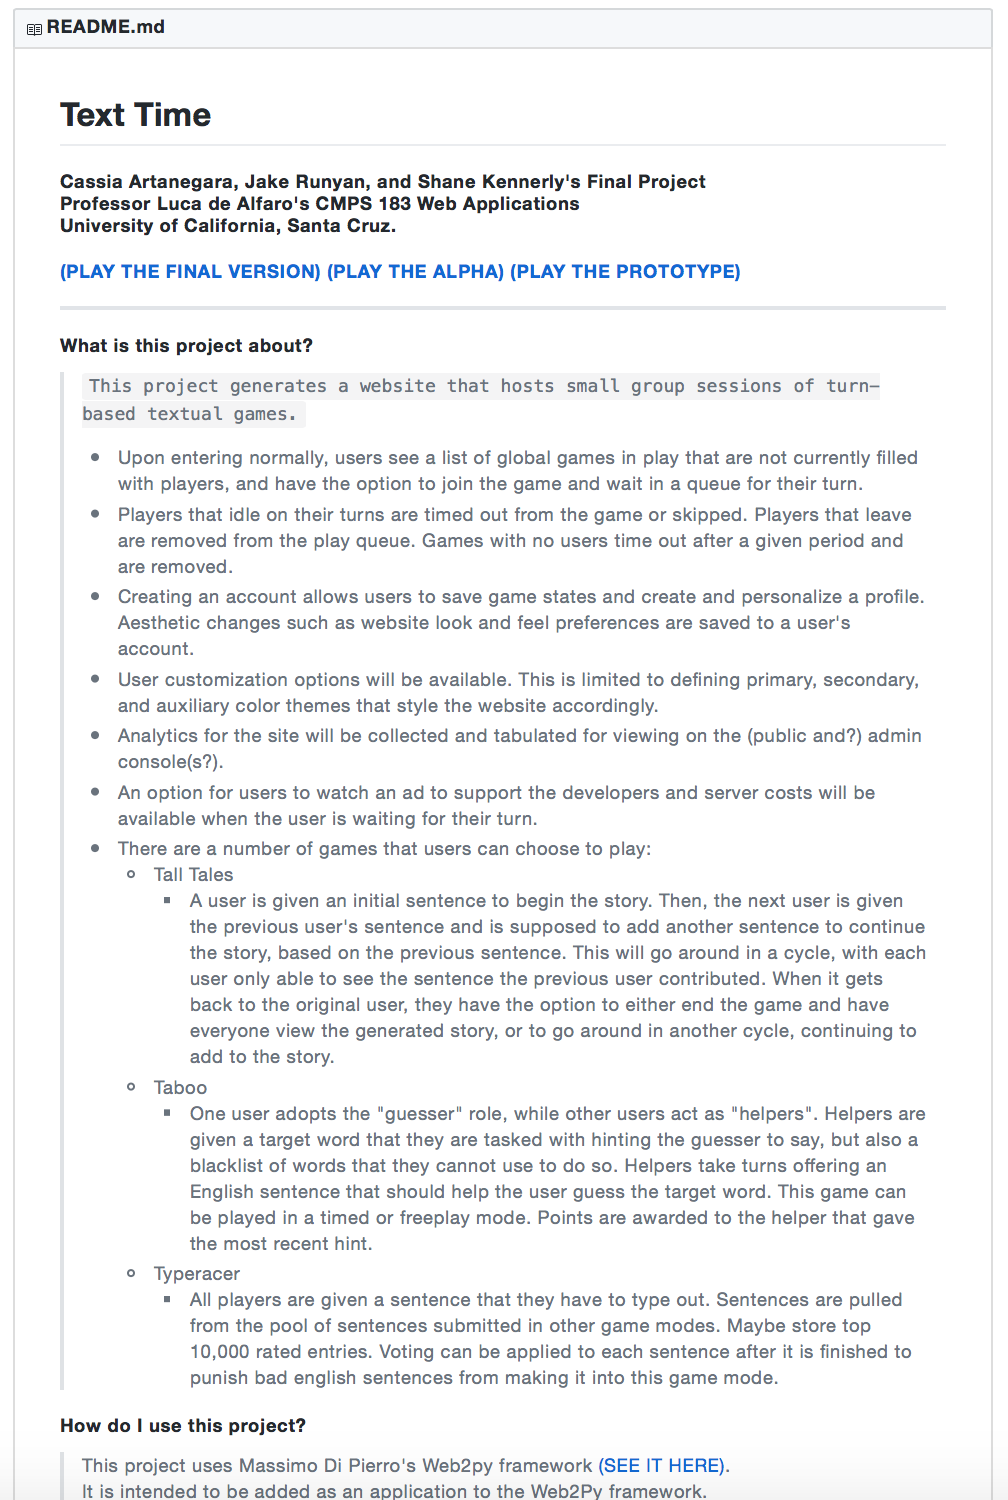
\includegraphics[width=200px]{data/readme.png}}
            \end{center}
        \end{figure}
    \end{frame}

    \begin{frame}
        \frametitle{Acknowledgements (Thank You!)}
        \begin{itemize}
          \item \textbf{The Web2py Team \& Massimo di Pierro, Lead Developer} for their framework
          \item \textbf{Luca de Alfaro \& teaching staff} for their instruction
          \item \textbf{Our peers} in CMPS 183 for their listening and time  
        \end{itemize}
    \end{frame}

    
\end{document}
    